%%%%% Preamble %%%%%
%\documentclass[a4paper,11pt]{article}
%\author{Walter Mottinelli}
%\title{Elaborazione numerica dei segnali con Scilab}
%\usepackage{latexsym}
%\usepackage{makeidx} % to generate indexes
%\usepackage[italian]{babel}
%\usepackage{ucs} % unicode encoding
%\usepackage[utf8]{inputenc}
%\usepackage{graphicx} % eps importing
%\pagestyle{headings}
%%%%%%%%%%%%%%%%%%%%
                                                                           
%\begin{document}
%\maketitle
%\tableofcontents
%\begin{abstract}
%\end{abstract}

\chapter{Trasformata $z$ e filtri digitali}
\section{Calcolo della funzione di trasferimento\ldots}
Nel dominio $z$, un sistema si comporta secondo la sua \emph{funzione di trasferimento}, cio\`e la trasformata $z$ della sua risposta all'impulso, quindi \`e importante poterla calcolare a partire dalle sequenze di ingresso e uscita o dalla equazione alle differenze.
\subsection*{\ldots\textrm{} date le sequenze di ingresso e di uscita}
Consideriamo ad esempio il filtro che converte la sequenza di ingresso
\begin{displaymath}
x(n)=r^n cos(\omega_0 n)
\end{displaymath}
(per $n \geq 0$) in \\
\begin{displaymath}
y(n)=r^n sen(\omega_0 n)
\end{displaymath}
(per $n \geq 0)$ e le loro trasformate \\
\begin{eqnarray*}
X(Z) & = & \frac{1-rcos(\omega_0)z^{-1}}{1-2rcos(\omega_0)z^{-1}r^2 z^{-2}} \\ 
Y(Z) & = & \frac{rsen(\omega_0)z^{-1}}{1-2rcos(\omega_0)z^{-1}r^2 z^{-2}}
\end{eqnarray*}
La funzione di trasferimento richiesta \`e data da 
\begin{eqnarray*}
H(z) & = & Y(z)/X(z) \\
     & = & \frac{rsen(\omega_0)z^{-1}}{1-rcos(\omega_0)z^{-1}}
\end{eqnarray*}
\subsection*{\ldots\textrm{} data l'equazione alle differenze}
Un sistema lineare tempo-invariante \`e descritto dalla seguente equazione alle differenze
\begin{displaymath}
y(n)=\sum_{k=1}^M a_k y(n-k) + \sum_{k=-N_F}^{N_P}b_k x(n-k)
\end{displaymath}
Prendiamone la trasformata $z$ e riordiniamone le sommatorie:
\begin{eqnarray*}
Y(z) & = & \sum_{n=-\infty}^{\infty} y(n)z^{-n} \\
     & = & \sum_{n=-\infty}^{\infty} \left [ \sum_{k=1}^M a_k y(n-k) + \sum_{k=-N_F}^{N_P} b_k x(n-k) \right] z^{-n} \\
     & = & \sum_{k=1}^M a_k \left [ \sum_{n=-\infty}^{\infty} y(n-k)z^{-n}\right ] + \sum_{k=-N_F}^{N_P} b_k \left [ \sum_{n=-\infty}^{\infty} x(n-k)z^{-n}\right ]
\end{eqnarray*}
Applicando la regola della trasformata $z$ di una sequenza ritardata, otteniamo
\begin{displaymath}
Y(z)=\sum_{k=1}^M a_k z^{-k}Y(z) + \sum_{k=-N_F}^{N_P} b_k z^{-k} X(z)
\end{displaymath}
Separiamo gli addendi contenenti $X(z)$ e $Y(z)$ e applichiamo la definizione della funzione di trasferimento $H(z)$: otteniamo il risultato atteso
\begin{displaymath}
H(z)=\frac{Y(z)}{X(z)}=\frac{\sum_{k=-{N_F}}^{N_P} b_k z^{-k}}{1- \sum_{k=1}^M a_k z^{-k}}
\end{displaymath}

\subsection*{Esempio di calcolo}
Consideriamo l'equazione alle differenze \\
\begin{displaymath}
y(n)=a_1 y(n-1)+a_2 y(n-2)+b_0 x(n)+b_1 x(n-1)
\end{displaymath}
Prendiamone la trasformata $z$
\begin{eqnarray*}
Y(z) & = & a_1z^{-1}Y(z)+a_2z^{-2}Y(z)+b_0 X(z)+b_1 z^{-1}X(z) \\
     & = & \frac{(b_0 + b_1 z^{-1})}{(1-a_1 z^{-1}-a_2 z^{-2})}X(z)
\end{eqnarray*}
La funzione di trasferimento \`e quindi 
\begin{displaymath}
H(z)=\frac{b_0 + b_1 z^{-1}}{1-a_1 z^{-1} -a_2 z^{-2}}
\end{displaymath}

\section{Disposizione di poli e zeri in un filtro generico}
Ricordiamo la scrittura della funzione di trasferimento come rapporto di due polinomi:
\begin{displaymath}
X(z)=\frac{P(z)}{Q(z)}
\end{displaymath}
Gli zeri, cio\`e i valori di $z$ per cui $P(z)=0$, indicano le frequenze complesse in cui il guadagno del filtro \`e nullo.
I poli, cio\`e i valori di $z$ per cui $Q(z)=0$, indicano le frequenze complesse in cui il guadagno del filtro \`e infinito.\\
Poli e zeri vicini all'origine non modificano significativamente la risposta in
frequenza del filtro, mentre zeri vicini alla circonferenza portano a zero le frequenze corrispondenti.\\
Se la ROC si estende oltre il polo pi\`u distante dal centro, allora il sistema \`e causale. Se la ROC include la circonferenza unitaria, allora il sistema \`e stabile. Ne segue che un filtro \`e causale e stabile se i poli sono tutti contenuti nel cerchio unitario.\\
Poich\'e ogni filtro pu\`o essere scomposto in filtri elementari di primo e secondo ordine, a loro volta distinguibili in ricorsivi e non ricorsivi, sono quattro le combinazioni base di poli e zeri:
\begin{itemize}
\item uno zero sull'asse reale in $z=r_0$ con $0 < r_0 < \infty$ e il polo corrispondente in $z=0$. La funzione di trasferimento del filtro non ricorsivo di prim'ordine che genera questa disposizione \`e 
\begin{displaymath}
H_1(z)=1-r_0 z^{-1}
\end{displaymath}
\item un polo sull'asse reale in posizione $z=r_0$ con $0 < r_0 < 1$ e il zero corrispondente in $z=0$. La funzione di trasferimento del filtro ricorsivo di prim'ordine che genera questa disposizione \`e 
\begin{displaymath}
H_2(z)=\left [1-r_0 z^{-1}\right ]^{-1}
\end{displaymath}
\item una coppia coniugata di zeri complessi in $z=r_0 e^{\pm i\omega_0}$ con $0 < r_0 < \infty$ e due poli corrispondenti in $z=0$. La funzione di trasferimento del filtro non ricorsivo di second'ordine che genera questa disposizione \`e 
\begin{displaymath}
H_3(z)=(1-r_0 e^{i\omega_0} z^{-1})(1-r_0 e^{-i\omega_0} z^{-1})=1-2r_0 cos(\omega_0)z^{-1}+r^2 z_0^{-2}
\end{displaymath}
\item una coppia coniugata di poli complessi in $z=r_0 e^{\pm i\omega_0}$ con $0 < r_0 < 1$ e due zeri corrispondenti in $z=0$. La funzione di trasferimento del filtro ricorsivo di second'ordine che genera questa disposizione \`e 
\begin{eqnarray*}
H_4(z) & = & \left[(1-r_0 e^{i\omega_0} z^{-1})(1-r_0 e^{-i\omega_0} z^{-1})\right ]^{-1} \\
       & = & \left[1-2r_0 cos(\omega_0)z^{-1}+r^2 z_0^{-2}\right]^{-1}
\end{eqnarray*}
\end{itemize}
In una funzione di trasferimento, gli zeri e i poli sono in numero uguale se vengono considerati anche i punti di singolarit\`a in $z=\infty$. Se, dopo aver analizzato i punti di singolarit\`a finiti, resta un disavanzo di $n$ zeri, significa che ci sono $n$ poli in $z=\infty$. La funzione di trasferimento di questa componente \`e 
\begin{displaymath}
H(5)=z^{n}
\end{displaymath}
ed \`e caratteristica dei sistemi non causali: la risposta all'impulso \`e anticipata di $n$ campioni. n caso di disavanzo di $n$ poli, si avranno $n$ zeri in $z=\infty$: la risposta all'impulso \`e ritardata di $n$ campioni.\\
La funzione di trasferimento complessiva di un filtro costituito da queste componenti \`e proporzionale al prodotto delle singole funzioni di trasferimento.

\subsection{Grafico della risposta in frequenza e in fase}

Mostriamo come poter ottenere con Scilab la risposta in frequenza e in fase di un filtro con funzione di trasferimento $H(z)=\frac{z}{z-a}$:

\begin{verbatim}
// zero della funzione di trasferimento del filtro
a=.5;
// creazione del numeratore
Ncoeff=[0,1];
N=poly(Ncoeff,'z','coeff');
// creazione del denominatore
Dcoeff=[-(a),1];
D=poly(Dcoeff,'z','coeff');
// definizione del range di frequenza
f=(0:.01:.5);
// calcolo della risposta in frequenza
hf=freq(N,D,exp(2*%pi*%i*f));
// settiamo la finestra per il grafico e lo visualizziamo
xbasc(); xset("font size",4);
xsetech([0,0,1,.5]); plot2d(f,(abs(hf)))
xtitle("Risposta in frequenza")
xsetech([0,.5,1,.5]); plot2d(f,atan(imag(hf),real(hf)));
xitle("Fase del filtro")
\end{verbatim}
Come risultato otteniamo il grafico rappresentato in figura \ref{Grafico_MagFase_1-2}.
%%%%%%%%%%%%%%%%%%%%%%%%%%%%
% Usage: -To include a Figure with a caption, insert the TWO following lines
%        in your Latex file:
% \input{This_file_name} 
% \dessin{The_caption}{The_label}
%         -To include just a picture, insert the lines 
%         between \fbox{\begin{picture}...  and \end{picture}} below 
%          
%%%%%%%%%%%%%%%%%%%%%%%%%%%%
 
 \long\def\Checksifdef#1#2#3{%
\expandafter\ifx\csname #1\endcsname\relax#2\else#3\fi}
\Checksifdef{Figdir}{\gdef\Figdir{}}{}
\def\dessin#1#2{
\begin{figure}[hbtp]
\begin{center}
%%%%%%%%%%%%%%%%%%%%%%%% 
%If you prefer cm, uncomment the following two lines
%\setlength{\unitlength}{1mm}
%\fbox{\begin{picture}(850.50,601.02)
%%%%%%%%%%%%%%%%%%%%%%%% 
\fbox{\begin{picture}(300.00,212.00)
%%%%%%%%%%%%%%%%%%%%%%%%%%%%%
% If you want to use epsfig, uncomment the following line 
% and comment the \special line 
%\epsfig{file=\Figdir Grafico_MagFase_1-2.eps,width=300.00pt,height=212.00pt}
%%%%%%%%%%%%%%%%%%%%%%%%%%%%%
\special{psfile=\Figdir Grafico_MagFase_1-2.eps hscale=100.00 vscale=100.00}
\end{picture}}
\end{center}
\caption{\label{#2}#1}
\end{figure}}

\dessin{Risposta in frequenza e in fase di $H(z)=\frac{z}{z-0,5}$}{Grafico_MagFase_1-2}
                                                                               
Al fine di evidenziare l'importanza del posizionamento degli zeri nel piano complesso $z$, riportiamo i grafici del modulo (figura \ref{Grafico_confronto_Mag}) e della fase (figura \ref{Grafico_confronto_Fase}) del filtro avente $H(z)=\frac{z}{z-a}$ per valori variabili dello zero $a$.
%%%%%%%%%%%%%%%%%%%%%%%%%%%%
% Usage: -To include a Figure with a caption, insert the TWO following lines
%        in your Latex file:
% \input{This_file_name} 
% \dessin{The_caption}{The_label}
%         -To include just a picture, insert the lines 
%         between \fbox{\begin{picture}...  and \end{picture}} below 
%          
%%%%%%%%%%%%%%%%%%%%%%%%%%%%
 
 \long\def\Checksifdef#1#2#3{%
\expandafter\ifx\csname #1\endcsname\relax#2\else#3\fi}
\Checksifdef{Figdir}{\gdef\Figdir{}}{}
\def\dessin#1#2{
\begin{figure}[htbp]
\begin{center}
%If you prefer cm use the following two lines
%\setlength{\unitlength}{1mm}
%\fbox{\begin{picture}(850.50,601.02)
\fbox{\begin{picture}(300.00,212.00)
% if you want to use epsfig uncomment the following line 
% and comment the special line 
%\epsfig{file=\Figdir Grafico_confronto_Mag.eps,width=300.00pt,height=212.00pt}
\special{psfile=\Figdir Grafico_confronto_Mag.eps hscale=100.00 vscale=100.00}
\end{picture}}
\end{center}
\caption{\label{#2}#1}
\end{figure}}

\dessin{Variazione della risposta in frequenza rispetto al valore dello zero (rosso=1.25; verde=0.75; blu=0.5; nero=0.25)}{Grafico_confronto_Mag}
%%%%%%%%%%%%%%%%%%%%%%%%%%%%
% Usage: -To include a Figure with a caption, insert the TWO following lines
%        in your Latex file:
% \input{This_file_name} 
% \dessin{The_caption}{The_label}
%         -To include just a picture, insert the lines 
%         between \fbox{\begin{picture}...  and \end{picture}} below 
%          
%%%%%%%%%%%%%%%%%%%%%%%%%%%%
 
 \long\def\Checksifdef#1#2#3{%
\expandafter\ifx\csname #1\endcsname\relax#2\else#3\fi}
\Checksifdef{Figdir}{\gdef\Figdir{}}{}
\def\dessin#1#2{
\begin{figure}[htbp]
\begin{center}
%If you prefer cm use the following two lines
%\setlength{\unitlength}{1mm}
%\fbox{\begin{picture}(850.50,601.02)
\fbox{\begin{picture}(300.00,212.00)
% if you want to use epsfig uncomment the following line 
% and comment the special line 
%\epsfig{file=\Figdir Grafico_confronto_Fase.eps,width=300.00pt,height=212.00pt}
\special{psfile=\Figdir Grafico_confronto_Fase.eps hscale=100.00 vscale=100.00}
\end{picture}}
\end{center}
\caption{\label{#2}#1}
\end{figure}}

\dessin{Variazione della fase rispetto al valore dello zero (rosso=1.25; verde=0.75; blu=0.5; nero=0.25)}{Grafico_confronto_Fase}


\section*{Disposizione di zeri e poli in un filtro a fase lineare}
Gli zeri di una funzione di trasferimento di un filtro lineare seguono una configurazione precisa.
Ricordando che un filtro \`e lineare se \`e simmetrico, scriviamo la stessa condizione nel dominio $Z$ e applichiamo la trasformata $z$:
\begin{eqnarray*}
h(n) & = & h(N-(1-n)) \\
H(z) & = & z^{-(N-1)H\left (\frac{1}{z}\right )}
\end{eqnarray*}
Ricordiamo che stiamo considerando un segnale ${h(n)}$ a valori reali: quindi, se $z_0$ \`e uno zero di $H(z)$, allora lo \`e anche il suo complesso coniugato $\bar{z_0}$; sfruttando la condizione di simmetria precedente, anche $\left (\frac{1}{z_0}\right )$ e $\left (\frac{1}{\bar{z_0}}\right )$ sono radici, quindi gli zeri generici di un filtro lineare esistono a gruppi di quattro.

\section{Progetto di filtri mediante disposizione \\iterativa di poli/zeri}
Lo scopo di questa sezione \`e di determinare la struttura di un filtro e dei suoi coefficienti posizionando in maniera iterativa poli e zeri nel piano $z$, osservando il risultato ottenuto dopo il loro posizionamento fino a quando non si realizza il filtro con le specifiche richieste.\\
Per semplificare la realizzazione del filtro si possono tener presente le seguenti regole e consigli:\\
\\
\emph{Regole}
\begin{itemize}
\item Le specifiche della risposta in frequenza consistono in regioni passa-banda e taglia-banda (vedi figura \ref{Prog-FiltroPB}). Queste bande sono mappate sulla circonferenza di raggio unitario con lo scopo di facilitare il posizionamento dei poli e degli zeri.
\item Tutti i poli dovranno avere un raggio $r_p$ compreso nell'intervallo \\$0,6\leq r_p<0,96$.\\
Il limite superiore garantisce che nella fase di realizzazione pratica eventuali errori di troncamento o arrotondamento causino l'instabilit\`a del filtro mentre il limite inferiore serve ad evitare di avere poli che diano una scarsa risposta in frequenza.
\item La progettazione del filtro viene ottimizzata analizzando, dopo ogni posizionamento di poli e zeri, il grafico della risposta in frequenza.\\
Operando in questo modo si pu\`o rimuovere la singolarit\`a o modificarne la posizione nel caso in cui non si ottenga l'effetto desiderato.
\end{itemize}
\emph{Consigli}
\begin{itemize}
\item Lo sviluppo dovrebbe iniziare posizionando un polo a distanza $r_p$ in mezzo ad ogni zona passa-banda e uno zero in mezzo ad ogni zona taglia-banda sulla circonferenza unitaria.
\item La risposta in frequenza al di sopra di una limitata banda di frequenze pu\`o essere incrementata inserendo, nella circonferenza di raggio unitario, un polo nell'angolo corrispondente al centro della banda interessata. La dimensione del raggio del polo determiner\`a l'aumento sia della banda sia del guadagno.
\item La risposta in frequenza al di sopra di una banda limitata pu\`o essere diminuita posizionando uno zero nell'angolo corrispondente al centro della banda. Per ottenere un'attenuazione massima, lo zero dovr\`a essere posizionato sulla circonferenza di raggio unitario.
\end{itemize}

\subsection{Realizzazione iterativa di un filtro passa-basso}
Proveremo ora a realizzare un filtro seguendo le indicazioni precedentemente citate.
Le caratteristiche del filtro passa-basso sono:\\
passa-banda
\begin{displaymath}
-1<|H(e^{j\omega})|_{dB}\leq0 \qquad\textrm{per } 0\leq\omega\leq\frac{\pi}{4}
\end{displaymath}
taglia-banda
\begin{displaymath}
|H(e^{j\omega})|_{dB}\leq-50 \qquad\textrm{per } \frac{\pi}{2}\leq\omega\leq\pi
\end{displaymath}

Le zone di interesse sono evidenziate nella figura \ref{Prog-FiltroPB}.\\
\begin{figure}[hp]
  \centering
  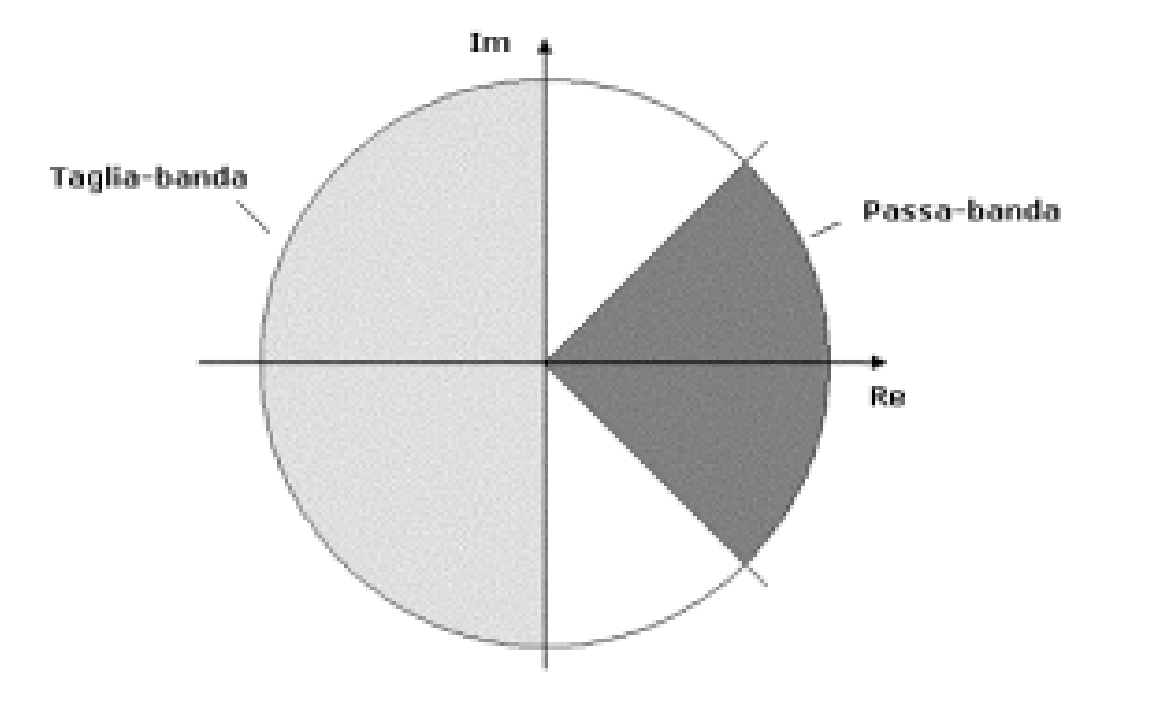
\includegraphics[scale=0.5]{images/Prog-FiltroPB.eps}
  \caption{Settori in cui verranno disposti i poli e gli zeri}
  \label{Prog-FiltroPB}
\end{figure}
%%%%%%%%%%%%%%%%%%%%%%%%%%%%%
% Usage: -To include a Figure with a caption, insert the TWO following lines
%        in your Latex file:
% \input{This_file_name} 
% \dessin{The_caption}{The_label}
%         -To include just a picture, insert the lines 
%         between \fbox{\begin{picture}...  and \end{picture}} below 
%          
%%%%%%%%%%%%%%%%%%%%%%%%%%%%
 
 \long\def\Checksifdef#1#2#3{%
\expandafter\ifx\csname #1\endcsname\relax#2\else#3\fi}
\Checksifdef{Figdir}{\gdef\Figdir{}}{}
\def\dessin#1#2{
\begin{figure}[htbp]
\begin{center}
%If you prefer cm use the following two lines
%\setlength{\unitlength}{1mm}
%\fbox{\begin{picture}(850.50,601.02)
\fbox{\begin{picture}(300.00,212.00)
% if you want to use epsfig uncomment the following line 
% and comment the special line 
%\epsfig{file=\Figdir Schema Filtro.eps,width=300.00pt,height=212.00pt}
\special{psfile=\Figdir Prog-FiltroPB.eps hscale=100.00 vscale=100.00}
\end{picture}}
\end{center}
\caption{\label{#2}#1}
\end{figure}}

%\dessin{Settori in cui verranno disposti i poli e gli zeri}{Prog-FiltroPB}

\subsubsection*{Passi della realizzazione}
\begin{itemize}
\item \emph{Singolarit\`a 1 e 2}\\
Posizionare un polo con raggio $r=0.7$ in mezzo alla zona passa-banda e uno zero in mezzo alla zona taglia-banda, sulla circonferenza unitaria.\\
La funzione di trasferimento del filtro risulta
\begin{displaymath}
H(z)=\frac{1+z^{-1}}{1-0,7z^{-1}}
\end{displaymath}
Il grafico della risposta in frequenza del filtro \`e rappresentato in figura \ref{RispFreq-Hz_sing1-2}.
%%%%%%%%%%%%%%%%%%%%%%%%%%%%
% Usage: -To include a Figure with a caption, insert the TWO following lines
%        in your Latex file:
% \input{This_file_name} 
% \dessin{The_caption}{The_label}
%         -To include just a picture, insert the lines 
%         between \fbox{\begin{picture}...  and \end{picture}} below 
%          
%%%%%%%%%%%%%%%%%%%%%%%%%%%%
 
 \long\def\Checksifdef#1#2#3{%
\expandafter\ifx\csname #1\endcsname\relax#2\else#3\fi}
\Checksifdef{Figdir}{\gdef\Figdir{}}{}
\def\dessin#1#2{
\begin{figure}[htbp]
\begin{center}
%If you prefer cm use the following two lines
%\setlength{\unitlength}{1mm}
%\fbox{\begin{picture}(850.50,601.02)
\fbox{\begin{picture}(300.00,212.00)
% if you want to use epsfig uncomment the following line 
% and comment the special line 
%\epsfig{file=\Figdir RispFreq-Hz_sing1-2.eps,width=300.00pt,height=212.00pt}
\special{psfile=\Figdir RispFreq-Hz_sing1-2.eps hscale=100.00 vscale=100.00}
\end{picture}}
\end{center}
\caption{\label{#2}#1}
\end{figure}}

\dessin{Risposta in frequenza del filtro dopo il posizionamento delle singolarit\`a 1 e 2}{RispFreq-Hz_sing1-2} 
\item \emph{Singolarit\`a 3} \\
Inserire uno zero in testa alla zona taglia-banda, sulla circonferenza unitaria.\\
La funzione di trasferimento del filtro risulta
\begin{displaymath}
H(z)=\frac{(1+z^{-1})(1+z^{-2})}{1-0,7z^{-1}}
\end{displaymath}
Il grafico della risposta in frequenza del filtro \`e rappresentato in figura \ref{RispFreq-Hz_sing3}.
%%%%%%%%%%%%%%%%%%%%%%%%%%%%
% Usage: -To include a Figure with a caption, insert the TWO following lines
%        in your Latex file:
% \input{This_file_name} 
% \dessin{The_caption}{The_label}
%         -To include just a picture, insert the lines 
%         between \fbox{\begin{picture}...  and \end{picture}} below 
%          
%%%%%%%%%%%%%%%%%%%%%%%%%%%%
 
 \long\def\Checksifdef#1#2#3{%
\expandafter\ifx\csname #1\endcsname\relax#2\else#3\fi}
\Checksifdef{Figdir}{\gdef\Figdir{}}{}
\def\dessin#1#2{
\begin{figure}[htbp]
\begin{center}
%If you prefer cm use the following two lines
%\setlength{\unitlength}{1mm}
%\fbox{\begin{picture}(850.50,601.02)
\fbox{\begin{picture}(300.00,212.00)
% if you want to use epsfig uncomment the following line 
% and comment the special line 
%\epsfig{file=\Figdir RispFreq-Hz_sing3.eps,width=300.00pt,height=212.00pt}
\special{psfile=\Figdir RispFreq-Hz_sing3.eps hscale=100.00 vscale=100.00}
\end{picture}}
\end{center}
\caption{\label{#2}#1}
\end{figure}}

\dessin{Risposta in frequenza del filtro dopo il posizionamento della singolarit\`a 3}{RispFreq-Hz_sing3}

\item \emph{Singolarit\`a 4} \\
Aggiungere un polo a $z=0,9e^{\pm j50^{\circ}}$ per sollevare la risposta in frequenza nella zona passa-banda.\\
La funzione di trasferimento del filtro risulta
\begin{displaymath}
H(z)=\frac{(1+z^{-1})(1+z^{-2})}{(1-0,7z^{-1})(1-1,16z^{-1}+0,81z^{-2})}
\end{displaymath}
Il grafico della risposta in frequenza del filtro \`e rappresentato in figura \ref{RispFreq-Hz_sing4}.
%%%%%%%%%%%%%%%%%%%%%%%%%%%%
% Usage: -To include a Figure with a caption, insert the TWO following lines
%        in your Latex file:
% \input{This_file_name} 
% \dessin{The_caption}{The_label}
%         -To include just a picture, insert the lines 
%         between \fbox{\begin{picture}...  and \end{picture}} below 
%          
%%%%%%%%%%%%%%%%%%%%%%%%%%%%
 
 \long\def\Checksifdef#1#2#3{%
\expandafter\ifx\csname #1\endcsname\relax#2\else#3\fi}
\Checksifdef{Figdir}{\gdef\Figdir{}}{}
\def\dessin#1#2{
\begin{figure}[htbp]
\begin{center}
%If you prefer cm use the following two lines
%\setlength{\unitlength}{1mm}
%\fbox{\begin{picture}(850.50,601.02)
\fbox{\begin{picture}(300.00,212.00)
% if you want to use epsfig uncomment the following line 
% and comment the special line 
%\epsfig{file=\Figdir RispFreq-Hz_sing4.eps,width=300.00pt,height=212.00pt}
\special{psfile=\Figdir RispFreq-Hz_sing4.eps hscale=100.00 vscale=100.00}
\end{picture}}
\end{center}
\caption{\label{#2}#1}
\end{figure}}

\dessin{Risposta in frequenza del filtro dopo il posizionamento della singolarit\`a 4}{RispFreq-Hz_sing4}

\item \emph{Singolarit\`a 5} \\
Posizionare uno zero sulla circonferenza unitaria, dove risulta massima la risposta nella zona taglia-banda. Questo zero limita l'incremento dovuto alla singolarit\`a 4.\\
La funzione di trasferimento del filtro risulta
\begin{displaymath}
H(z)=\frac{(1+z^{-1})(1+z^{-2})(1+1,03z^{-1}+z^{-2})}{(1-0,7z^{-1})(1-1,16z^{-1}+0,81z^{-2})}
\end{displaymath}
Il grafico della risposta in frequenza del filtro \`e rappresentato in figura \ref{RispFreq-Hz_sing5}.
%%%%%%%%%%%%%%%%%%%%%%%%%%%%
% Usage: -To include a Figure with a caption, insert the TWO following lines
%        in your Latex file:
% \input{This_file_name} 
% \dessin{The_caption}{The_label}
%         -To include just a picture, insert the lines 
%         between \fbox{\begin{picture}...  and \end{picture}} below 
%          
%%%%%%%%%%%%%%%%%%%%%%%%%%%%
 
 \long\def\Checksifdef#1#2#3{%
\expandafter\ifx\csname #1\endcsname\relax#2\else#3\fi}
\Checksifdef{Figdir}{\gdef\Figdir{}}{}
\def\dessin#1#2{
\begin{figure}[htbp]
\begin{center}
%If you prefer cm use the following two lines
%\setlength{\unitlength}{1mm}
%\fbox{\begin{picture}(850.50,601.02)
\fbox{\begin{picture}(300.00,212.00)
% if you want to use epsfig uncomment the following line 
% and comment the special line 
%\epsfig{file=\Figdir RispFreq-Hz_sing5.eps,width=300.00pt,height=212.00pt}
\special{psfile=\Figdir RispFreq-Hz_sing5.eps hscale=100.00 vscale=100.00}
\end{picture}}
\end{center}
\caption{\label{#2}#1}
\end{figure}}

\dessin{Risposta in frequenza del filtro dopo il posizionamento della singolarit\`a 5}{RispFreq-Hz_sing5}

\item \emph{Singolarit\`a 6} \\
Aggiungere un polo in $z=0,75e^{\pm j40^{\circ}}$ per incrementare la risposta in frequenza in testa alla zona passa-banda.\\
La funzione di trasferimento del filtro risulta
\begin{displaymath}
H(z)=\frac{(1+z^{-1})(1+z^{-2})(1+1,03z^{-1}+z^{-2})}{(1-0,7z^{-1})(1-1,16z^{-1}+0,81z^{-2})(1-1,15z^{-1}+0,56z^{-2})}
\end{displaymath}
Il grafico della risposta in frequenza del filtro \`e rappresentato in figura \ref{RispFreq-Hz_sing6}.
%%%%%%%%%%%%%%%%%%%%%%%%%%%%
% Usage: -To include a Figure with a caption, insert the TWO following lines
%        in your Latex file:
% \input{This_file_name} 
% \dessin{The_caption}{The_label}
%         -To include just a picture, insert the lines 
%         between \fbox{\begin{picture}...  and \end{picture}} below 
%          
%%%%%%%%%%%%%%%%%%%%%%%%%%%%
 
 \long\def\Checksifdef#1#2#3{%
\expandafter\ifx\csname #1\endcsname\relax#2\else#3\fi}
\Checksifdef{Figdir}{\gdef\Figdir{}}{}
\def\dessin#1#2{
\begin{figure}[htbp]
\begin{center}
%If you prefer cm use the following two lines
%\setlength{\unitlength}{1mm}
%\fbox{\begin{picture}(850.50,601.02)
\fbox{\begin{picture}(300.00,212.00)
% if you want to use epsfig uncomment the following line 
% and comment the special line 
%\epsfig{file=\Figdir RispFreq-Hz_sing6.eps,width=300.00pt,height=212.00pt}
\special{psfile=\Figdir RispFreq-Hz_sing6.eps hscale=100.00 vscale=100.00}
\end{picture}}
\end{center}
\caption{\label{#2}#1}
\end{figure}}

\dessin{Risposta in frequenza del filtro dopo il posizionamento della singolarit\`a 6}{RispFreq-Hz_sing6}

\item \emph{Singolarit\`a 7} \\
Posizionare un polo in $z=0,6e^{\pm j38^{\circ}}$ per incrementare la risposta in frequenza in mezzo alla zona passa-banda.\\
\end{itemize}
La funzione di trasferimento finale del filtro risulta
\begin{displaymath}
\textstyle
H(z)=\frac{(1+z^{-1})(1+z^{-2})(1+1,03z^{-1}+z^{-2})}{(1-0,7z^{-1})(1-1,16z^{-1}+0,81z^{-2})(1-1,15z^{-1}+0,56z^{-2})(1-0,95z^{-1}+0,36z^{-2})}
\end{displaymath}
Alla funzione di trasferimento del filtro bisogna aggiungere un guadagno pari a $0,0027$; questo valore permette di normalizzare il guadagno.

\subsubsection*{Grafico finale della risposta in frequenza}
Per realizzare il grafico con Scilab si possono utilizzare i seguenti comandi
\begin{verbatim}
// definiamo il numeratore della funzione di traferimento
num_Hz=(1+%z^(-1))*(1+%z^(-2))*(1+1.03*%z^(-1)+%z^(-2));
// fattorizziamo il lungo denominatore in tre termini
den1_Hz=(1-0.7*%z^(-1))*(1-1.16*%z^(-1)+0.81*%z^(-2));
den2_Hz=(1-1.15*%z^(-1)+0.56*%z^(-2));
den3_Hz=(1-0.95*%z^(-1)+0.36*%z^(-2);
// componiamo il denominatore
den_Hz=den1_Hz*den2_Hz*den3_Hz;
// infine creiamo la funzione di trasferimento
Hz=num_Hz/den_Hz;
A=0.0027;
// calcoliamo la risposta in frequenza
[xm,fr]=frmag(A*Hz,100);
// Disegna il grafico del modulo della risposta in frequenza
plot2d(fr,xm);
xtitle(xtit="",xax="frequenza",yax="|H(w)|");
xset("line style",3);
y=(0:100);
xt=(.125*ones(y));
// Disegna la frequenza di taglio
plot2d(xt,y,rect=[0,0,.5,1],style=(3),leg="frequenza taglio");
xs=(.25*ones(y));
// Disegna la frequenza di stop
plot2d(xs,y,rect=[0,0,.5,1],style=(5));
\end{verbatim}
Il grafico finale della risposta in frequenza del filtro \`e rappresentato in figura \ref{RispFreq-Hz_finale}.
%%%%%%%%%%%%%%%%%%%%%%%%%%%%
% Usage: -To include a Figure with a caption, insert the TWO following lines
%        in your Latex file:
% \input{This_file_name} 
% \dessin{The_caption}{The_label}
%         -To include just a picture, insert the lines 
%         between \fbox{\begin{picture}...  and \end{picture}} below 
%          
%%%%%%%%%%%%%%%%%%%%%%%%%%%%
 
 \long\def\Checksifdef#1#2#3{%
\expandafter\ifx\csname #1\endcsname\relax#2\else#3\fi}
\Checksifdef{Figdir}{\gdef\Figdir{}}{}
\def\dessin#1#2{
\begin{figure}[htbp]
\begin{center}
%If you prefer cm use the following two lines
%\setlength{\unitlength}{1mm}
%\fbox{\begin{picture}(850.50,601.02)
\fbox{\begin{picture}(300.00,212.00)
% if you want to use epsfig uncomment the following line 
% and comment the special line 
%\epsfig{file=\Figdir RispFreq-Hz_finale.eps,width=300.00pt,height=212.00pt}
\special{psfile=\Figdir RispFreq-Hz_finale.eps hscale=100.00 vscale=100.00}
\end{picture}}
\end{center}
\caption{\label{#2}#1}
\end{figure}}

\dessin{Risposta in frequenza finale del filtro.}{RispFreq-Hz_finale}

\subsubsection*{Grafico finale dei poli e degli zeri}
Per realizzare il grafico con Scilab si possono utilizzare i seguenti comandi
\begin{verbatim}
// Grafico poli/zeri
num_Hz=(1+%z^(-1))*(1+%z^(-2))*(1+1.03*%z^(-1)+%z^(-2)); 
// fattorizziamo il lungo denominatore in tre termini
den1_Hz=(1-0.7*%z^(-1))*(1-1.16*%z^(-1)+0.81*%z^(-2));
den2_Hz=(1-1.15*%z^(-1)+0.56*%z^(-2));
den3_Hz=(1-0.95*%z^(-1)+0.36*%z^(-2);
// componiamo il denominatore 
den_Hz=den1_Hz*den2_Hz*den3_Hz;
Hz=num_Hz/den_Hz;
xbasc(); plzr(Hz)
\end{verbatim}
Il grafico dei poli/zeri del filtro \`e rappresentato in figura \ref{Grafico_Poli-Zeri}.
%%%%%%%%%%%%%%%%%%%%%%%%%%%%
% Usage: -To include a Figure with a caption, insert the TWO following lines
%        in your Latex file:
% \input{This_file_name} 
% \dessin{The_caption}{The_label}
%         -To include just a picture, insert the lines 
%         between \fbox{\begin{picture}...  and \end{picture}} below 
%          
%%%%%%%%%%%%%%%%%%%%%%%%%%%%
 
 \long\def\Checksifdef#1#2#3{%
\expandafter\ifx\csname #1\endcsname\relax#2\else#3\fi}
\Checksifdef{Figdir}{\gdef\Figdir{}}{}
\def\dessin#1#2{
\begin{figure}[hbtp]
\begin{center}
%%%%%%%%%%%%%%%%%%%%%%%% 
%If you prefer cm, uncomment the following two lines
%\setlength{\unitlength}{1mm}
%\fbox{\begin{picture}(850.50,601.02)
%%%%%%%%%%%%%%%%%%%%%%%% 
\fbox{\begin{picture}(300.00,212.00)
%%%%%%%%%%%%%%%%%%%%%%%%%%%%%
% If you want to use epsfig, uncomment the following line 
% and comment the \special line 
%\epsfig{file=\Figdir Grafico_Poli-Zeri.eps,width=300.00pt,height=212.00pt}
%%%%%%%%%%%%%%%%%%%%%%%%%%%%%
\special{psfile=\Figdir Grafico_Poli-Zeri.eps hscale=100.00 vscale=100.00}
\end{picture}}
\end{center}
\caption{\label{#2}#1}
\end{figure}}

\dessin{Grafico poli/zeri del filtro.}{Grafico_Poli-Zeri}

%\end{document}
